% Eingangsdaten der Simulation

\section{Modelleingangsdaten}

Grundlage für die Lastflussberechnung durch \edisgo bilden verschiedene Modelleingangsdaten.
Hierzu gehören in erster Linie die mit \simbev erzeugten Lastprofile der Ladevorgänge der \gls{EPKW}, sowie die Erzeugungsprofile erneuerbarer Energieanlagen in einem Netzgebiet.
Weiterhin gehen auch die Lastprofile von Wärmepumpen in die Lastflussberechnung mit ein.

\subsection{Erzeugung der Lastzeitreihen der Ladevorgänge von E-Pkw}

Mit Hilfe des im Rahmen dieser Masterarbeit mitentwickelten Software Tools \simbev können die Fahrtprofile für eine beliebige Anzahl an Fahrzeugen der verschiedenen Klassen für einen Regionstypen erstellt werden.
Die Fahrtprofile enthalten die gefahrenen Strecken und die Standzeiten am Zielort.
Aus diesen können anschließend anhand des Verbrauchs und der gegebenen Ladeinfrastruktur die Ladebedarfe am Zielort abgeleitet werden.
Abhängig von der Ladestrategie wird innerhalb der Standzeit die Last auf die Standzeit verteilt.
Die Zeitreihen der Ladelast der einzelnen Fahrzeuge werden innerhalb eines Landkreises berechnet und schlussendlich zu einer Gesamtlast je \UC zusammengeführt.
Mit Hilfe des proprietär \localiserToolsKomma , werden die Zeitreihen der Gesamtlasten auf konkrete georeferenzierte Ladepunkte innerhalb des Landkreises verteilt.
Um abschließend eine Lasflussrechnung eines Netzgebietes mit \edisgo durchführen zu können, muss die Schnittmenge eines Netzgebietes mit den Landkreisen bestimmt werden.
Ladepunkte die innerhalb dieser Schnittmenge liegen, werden dem jeweiligen Netzgebiet zugeordnet und somit die entsprechende Last der Ladevorgänge.

\subsubsection{Erzeugung der Fahrtprofile mit simbev}

% TODO: Regionstypen erklären RegioStaR7

Die Fahrtprofile werden über einen pro­ba­bi­lis­tischen Ansatz mit Hilfe des im Rahmen dieser Masterarbeit mitentwickelten Software Tools \simbev erzeugt.
Die Grundlage des pro­ba­bi­lis­tischen Ansatzes bildet die Befragung \gls{MID} \cite{ISGH2017}.
Dabei erhält jeder simulierte Zeitschritt eine Wahrscheinlichkeit für einen bestimmten Wegezweck eine Fahrt zu beginnen.
Löst ein Fahrzeug eine Fahrt aus, wird abhängig vom Wegezweck und Regionstyp der Fahrt ebenfalls pro­ba­bi­lis­tisch eine Streckenlänge und eine anschließende Standzeit zugeordnet.
Der hierbei entstehende Verbrauch des Fahrzeuges muss anschließend gedeckt werden.
Ob am Zielort ein Ladevorgang stattfindet, hängt vom \gls{SOC} des Fahrzeuges und dem vorhandensein eines Ladepunktes ab.
Ob ein Ladepunkt am Zielort zur Verfügung steht und welche Ladeleistung dieser aufweist, wird mit Hilfe der Wahrscheinlichkeiten aus \autoref{tab:WegezweckProbability2035} bzw. \autoref{tab:WegezweckProbability2050} ermittelt.
Die Bestimmung des vorhandenseins eines Ladepunktes zu Hause und am Arbeitsplatz erfolgt je \gls{EPKW} einmalig und wird anschließend konstant gehalten.
Für alle anderen Wegezwecke, erfolgt die Bestimmung kontinuierlich.
Wurde dem Zielort ein Ladepunkt zugeordnet wird davon ausgegangen, dass der Fahrzeugnutzer einen Ladevorgang erst ab einem bestimmten \gls{SOC} einleitet, da dies einen zusätzlichen Aufwand für den Nutzer bedeutet.
Dabei wird angenommen, dass das Laden des Fahrzeuges am Wohnort und am Arbeitsplatz bereits ab einem \gls{SOC} von \SI{95}{\percent} stattfindet.
Im öffentlichen Raum bedeutet das Anfahren und der Anschluss an einen Ladepunkt einen größeren Aufwand für den Nutzer als im privaten Raum.
Deshalb wird angenommen, dass oberhalb eines \glspl{SOC} von \SI{80}{\percent} keine Ladevorgänge stattfinden.
Es gilt je niedriger der \gls{SOC}, desto wahrscheinlicher ist es, dass die öffentliche Ladeinfrastruktur genutzt wird.
Ab einem \gls{SOC} von \SI{50}{\percent} findet, wann immer möglich, eine Ladung des Fahrzeugs statt.
Zwischen den beiden Stützwerten erfolgt eine lineare Interpolation, welche in \autoref{fig:soc_charging_prob} visualisiert wurde.

\begin{figure}[H]
    \centering
    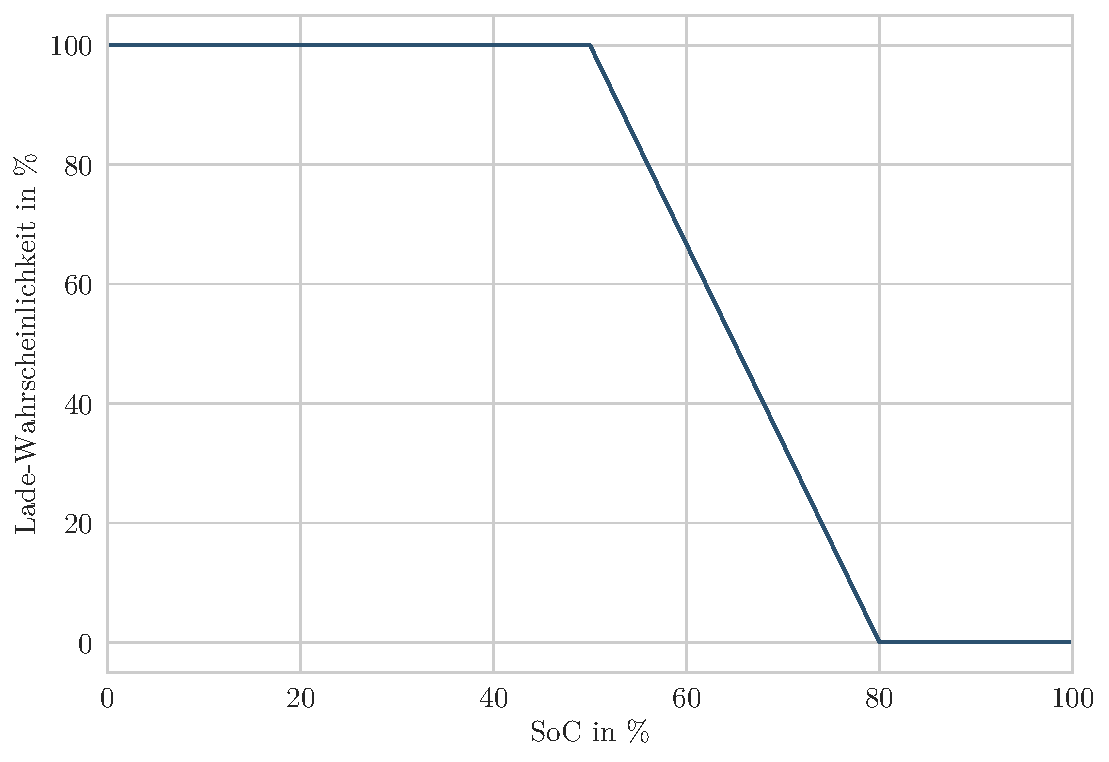
\includegraphics[width=\textwidth]{Bilder/soc_charging_prob}
    \caption{Abhängigkeit der Ladewahrscheinlichkeit vom SoC an öffentlichen Standorten}\label{fig:soc_charging_prob}
\end{figure}

Schnellladeinfrastruktur besitzt aufgrund des zusätzlichen Fahrt- und Zeitaufwandes eine geringe Attraktivität für den Nutzer.
Deshalb wird eine Schnellladung in dieser Simulation nur dann ausgelöst, wenn es wirklich nötig ist.
Sinkt der \gls{SOC} eines Fahrzeugs unter \SI{15}{\percent}, wird eine Schnellladestation angefahren und das Fahrzeug wird für \SI{15}{\Minuten} geladen.
Im Unterschied zu \glspl{BEV}, können \glspl{PHEV} auch mit einem \gls{SOC} von \SI{0}{\percent} ihre Fahrt mit Hilfe des Verbrennungsmotors fortsetzen.
Aus diesem Grund wird bei \glspl{PHEV} kein Schnellladevorgang ausgelöst.

\subsubsection{Regionalisierung}

Die Regionalisierung der Fahrzeuge auf die Landkreise findet auf Grundlage des Fahrzeugbestandes nach Zulassungsbezirken \cite[][Stand: \DTMdate{2020-01-01}]{KBAPLZ2020} statt.
Es wird davon ausgegangen, dass es zu keiner Verschiebung des Anteils am Bestand zwischen den Zulassungsbezirken kommt.
Dies bedeutet, dass die Gesamtanzahl der Fahrzeuge je Fahrzeugklasse je Szenario entsprechend des heutigen Bestandes anteilig verteilt wird.

\subsubsection{Implementierung der Ladestrategien in simbev}

\subsubsection{Localiser Tool}